\documentclass[conference,11pt]{IEEEtran}
\usepackage[utf8]{inputenc}
\usepackage[english]{babel}
\usepackage[left=1in,right=1in,top=1in,bottom=1in,footskip=.25in]{geometry}
\usepackage{cite}
\usepackage{hyperref}
\usepackage{fancyhdr}
\usepackage{datetime}
\usepackage{amsmath}
\usepackage{url}
\usepackage{subfig}
\usepackage{float}
\usepackage{graphicx}
\graphicspath{ {images/} }
\usepackage{setspace}
%\setlength{\parskip}{1em}
\pagenumbering{arabic}
\pagestyle{fancy}

\usepackage[numbered,framed]{matlab-prettifier}
\usepackage[T1]{fontenc}
\usepackage[scaled]{beramono}
\lstset{
  style              = Matlab-editor,
  basicstyle         = \mlttfamily,
  escapechar         = ",
  mlshowsectionrules = true,
}

\title{Feature Transfer Learning for Automated Lung Cancer Detection}
\author{
    \IEEEauthorblockN{Benjamin Hillmann}
    \IEEEauthorblockA{
        \today
    }
}

\begin{document}
\onecolumn
\maketitle

\begin{abstract}
In order to assess early risk factors of high-risk patients for lung cancer, a non-invasive low-resolution computed tomography (CT) scan is administered. The results of the CT scan are a 3D intensity image of the patients chest region. The important features of this scan are nodules or masses within the lungs, that can be classified as either benign (non-cancerous) or malignant (cancerous). Typically, a radiologist will analyze the scans to determine the diagnosis of the nodules and the patient. With advances in technology, experiments are being conducted with computer-aided diagnosis (CAD) technologies to synergize with human expertise analysis and reduce false positive diagnosis. In this work, abstract image features from deep neural networks are extracted from each slice of the CT scan. These abstract features are then combined and their correlation and prediction capabilities for malignancy are assessed.
\end{abstract}

\section{Introduction}

Cancer is one of the leading causes of death worldwide, accounting for 8.8 million deaths in the year 2015 \cite{noauthor_who_nodate}. Within the United States, lung cancer is the deadliest form as shown in \textit{Figure ~\ref{fig:cancer}} and costs billions in dollars in health care costs \cite{noauthor_united_nodate}. With current medicine technologies, many of the current cases of lung cancer can be prevented. Prevention techniques can be implemented through avoiding risk factors, raising awareness of prevention strategies, and early stage detection and management of cancer patients.

Early detection and diagnosis of cancer can reduce the mortality rate of cancer. A common early stage detection technique is to administer a low-resolution computed tomography (CT) scan for high-risk patients. Some of the benefits of CT scans include they are non-invasive and low-risk to administer. The CT scans produce 3D mass intensity image of the patients chest region. The important features of this scan are detecting nodules or masses within the lungs, that can be classified as either benign (non-cancerous) or malignant (cancerous). Typically, a radiologist will analyze the scans to determine the diagnosis of the nodules and the patient. With advances in technology, experiments are being conducted with computer-aided diagnosis (CAD) technologies to synergize with human expertise analysis and reduce false positive diagnosis.

The purpose of this analysis is to develop CAD classification algorithms to classify lesions in the lung from CT scans as being cancerous. The input for the classifiers are 3D intensity scans of the upper chest region of high-risk patients. The output of the classifier is the risk that the patient will develop lung cancer within the next year. The state of the art algorithms in computer vision and machine learning described in this analysis reduces the number of false positive diagnosis made by current CAD technology \cite{sun_automatic_2017}. The successfulness of this approach will allow patients to receive quicker access to life-saving intervention, and give radiologists more time to provide that intervention.

The approach outlined in this paper is an experiment in the transferability of abstract features learned within the inner layers of a deep neural network. An original deep neural network was trained on the semantic tags given to the natural image database Imagenet \cite{russakovsky_imagenet_2015,yosinski_how_2014,he_deep_2015}. The classification layers are removed from the original network, and the weights output from the remaining layers are treated as the input feature space. The abstract features are averaged across all layers in the image, and the resulting embedding is input to a gradient boosting machine. Analysis of the method shows that the proposed methods outperforms a random and majority class classifier. Furthermore, the specific feature space outperforms a boosting gradient machine on a random feature space. This approach shows the effectiveness of the generalization of feature embeddings provided by deep neural networks trained in non-related domains to targeted problems. This approach is generally useful when the number of samples to train is relatively low due to complexities or cost of dataset collection, such as with biomedical datasets.

%%% fig:cancer
\begin{figure}
    \centering
    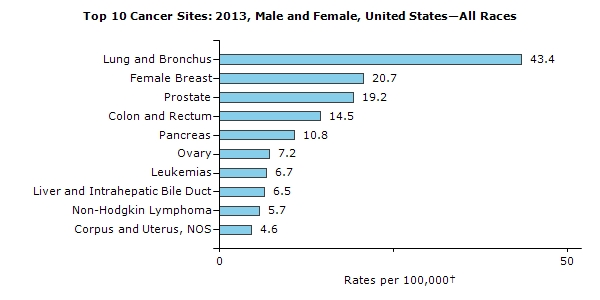
\includegraphics[width=0.8\linewidth]{figures/plot_top_ten_cancers.jpg}
    \caption{Death rates of the most common forms of cancer in the United States per 100,000 people. Lung and bronchus cancer has the highest mortality rate, with more than twice the mortality rate of the second deadliest form of cancer.}
      \label{fig:cancer}
\end{figure}

\section{Background}

The goal for this project was to apply techniques in ongoing machine learning and artificial intelligence research to accurately predict the risk for a patient to develop lung cancer \cite{ronneberger_u-net:_2015}. This project was an entry into the Data Science Bowl, an annual competition hosted by the data science competition website  \href{https://www.kaggle.com/c/data-science-bowl-2017}{Kaggle}. This competitions aligns with the Cancer Moonshot initiative, with the goal of utilizing intelligent data analysis to advance screening, care and prevention of cancer. The endgame of the initiative is to end the disease entirely.

\subsection{Dataset}
The data for this project is being hosted by the data science competition website \href{https://www.kaggle.com/c/data-science-bowl-2017}{Kaggle} as a part of the 2017 Science Bowl. The data includes over a thousand low-dose CT images from patients that are high-risk for lung cancer. The format they are provided in is DICOM, and contains 3D segmented intensity scans of various resolutions.

%%% dataset
\begin{figure}[]
    \centering
    \[
      \begin{array} {|c|c|c|c|c|}
        \hline
        & \textnormal{Train Set} & \textnormal{Test Set} & \textnormal{Size (GB)} & \textnormal{Size Compressed (GB)} \\ \hline
        \textnormal{stage1}  & 1398 & 199 & 139 & 112 \\ \hline
        \textnormal{stage2}  & 0 & 507 & 91.1 & 69.5\\ \hline
      \end{array}
    \]
    \caption{Summary statistics for the number of samples and disk used for the competition dataset. The stage1 of the competition was used for evaluation and submission of the models. The stage2 was for final evaluation of the competition to show the generalization of the models, to guard against information leakage, leaderboard hacking, and over-training. File compression was enabled on the hard drive to reduce space and show the redundancy in the data.}
    \label{fig:dataset}
\end{figure}

The competition was formatted in two stages. The first stage, labeled as stage1, was designed to build and test models. The data for stage1 was separated into a training, meaning labeled with being cancerous or not, and a test set containing no labels. A competitor would download all the data for stage1, build a supervised machine learning regression on the training set, then upload their predictions for the stage1 test set to the website leaderboard. The input for the computational pipeline was the DICOM images, and the output target was the risk $y$ in the range $y \in (0,1)$ that a patient develops lung cancer in the next year. The leaderboard was ordered by submissions with the lowest LogLoss on the training set. The LogLoss of the test set is defined below:

%%% LogLoss
$$ \textrm{LogLoss} = - \frac{1}{n} \sum_{i=1}^n \left[ y_i \log(\hat{y}_i) + (1 - y_i) \log(1 - \hat{y}_i)\right]. $$

The second stage of the competition, labeled as stage2, contained no labeled training data. The purpose of stage2 was to reduce over-training on the dataset, eliminate leaderboard hacking of various submission for better scores, and to evaluate the bias in each of the submissions. There is a public and a private leaderboard in stage2. The public leaderboard was a small and unknown subsample of the stage2 test data. The private leaderboard contained the rest of the testing data not included in the public leaderboard and was used for the final evaluation of the submissions based on LogLoss. The sample size and disk usage for each of the stages are shown in \textit{Figure ~\ref{fig:dataset}}.

\subsection{Deep Neural Networks for Image Classification}

Deep neural networks have been utilized for breakthrough results in image classification \cite{he_deep_2015}. For example, consider the problem of semantic tagging and the Imagenet 2012 dataset \cite{russakovsky_imagenet_2015}. Semantic tagging is the process of annotating an image with keywords that appeared in that image. In the ImageNet 2012 dataset,  there are 1.28 million training images with human annotated 1,000 classes or semantic tags. There are 50k validation images, with the objective of automatically tagging these images with as little error as possible. An example image and classification using a deep neural network is shown in \textit{Figure ~\ref{fig:elephant}}.  The architecture of deep neural networks allows the combination of low, mid and high level image features that are enriched by many stacked layers. These neural networks have been shown, when properly tuned, to provide the best end-to-end solution with the lowest error for semantic tagging on the Imagenet dataset. 

%%% elephant
\begin{figure}
    \centering
      \subfloat[] {
         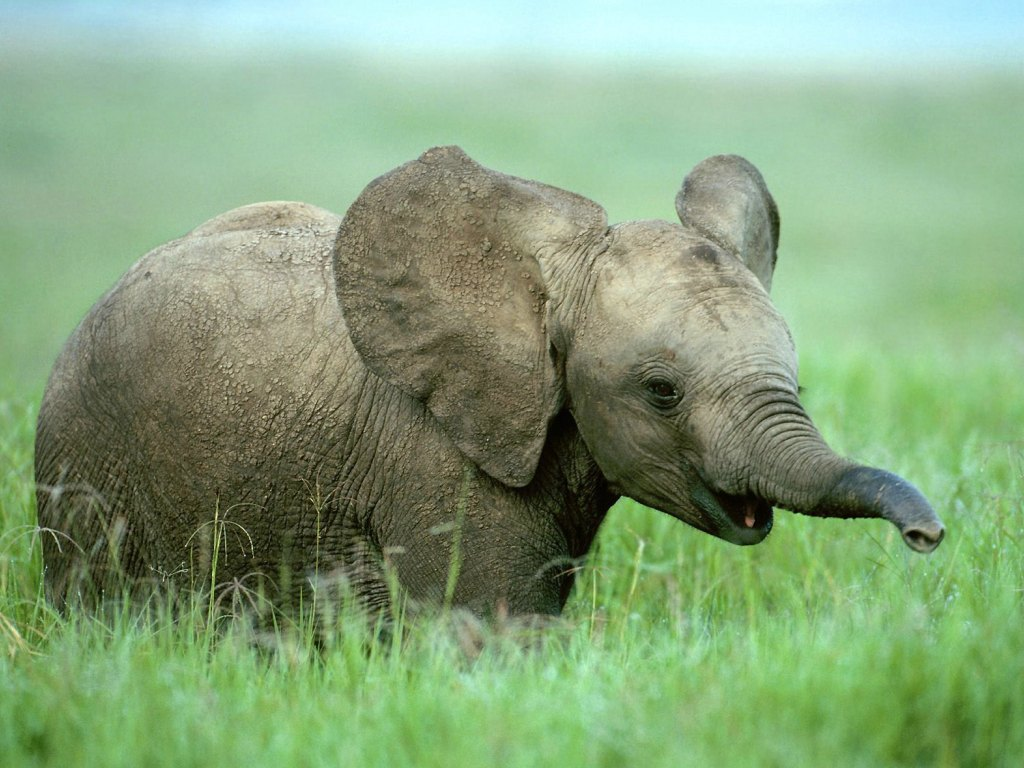
\includegraphics[width=0.4\linewidth]{figures/plot_elephant.jpg}
      }
    	\hspace{0.02\linewidth}
      \subfloat[]{
          \begin{tabular} {|c|c|}
            \hline
            \textnormal{Semantic Tag} & \textnormal{Similarity} \\ \hline
           139 & 112 \\ \hline
           91.1 & 69.5\\ \hline
          \end{tabular}
      }
      \caption{Displaying the original.}
      \label{fig:elephant}
\end{figure}

\subsection{Nodule Segmentation}

Previous work for risk regression using CAD has been focused around image segmentation. In the case of lung cancer, the 3D images are segmented into voxels that contain nodules. Nodules are small masses within the lung, and their properties such as shape and size are what human annotators use for diagnosing cancer risk. For this task, a specific architecture of a convolution neural network (CNN) has been trained to detect nodules given an image \cite{ronneberger_u-net:_2015}. The training set size $N$ for this network architecture are assumed to be small, $10 < N < 10,000$. The training set utilized in this paper contained radiologist segmented images that are cut around nodules. The network is designed to maximize the trade-off between classifier localization and context accuracy. Localization is the ability of the classifier to correctly label each pixel of an image as containing a nodule or not. The contextual accuracy is the ability to predict each group of pixels accordingly as a nodule, that is, the number of nodules detected is correct. The network architecture describes meets these goals by a dual channel approach, with one channel being traditional convolution operations for contextual features, and the second channel being an up-sampling architecture for pixel localization.

After an image is segmented, properties of each individual voxel is regressed towards being malignant. Often times, after nodule segmentation of an image is complete, there exists many false positive candidate nodules. An approach to increase precision to utilize a graph cutting algorithm followed by a CNN architecture specifically designed to reduce false positives \cite{sun_automatic_2017}. After false positive reduction, the final candidate nodules are analyzed by a CNN to predict malignancy.

\subsection{Transfer Learning}

The first few layers of deep neural networks trained on natural images tend to lend themselves to the same phenomena, they learn color blobs and abstract edge filters \cite{yosinski_how_2014}. These features do not limit themselves to particular tasks or datasets and nevertheless are common between many of them. Therefore, when the sample size for a particular dataset is small, it is often the case that these first few layers of a previously learned dataset can be transferred successfully as the initialization weights for a new classification task. The transferability of these edge weights heave been shown to rely on two issues. The first is the specialization of layers to their original task. The second is the optimization of co-adapted layers that were split from the original network. Even with these issues, often times the transferability of these weights lends itself to fast stabilization of new classification tasks. The transferability of features also decreases as the difference between the original task and the target task increases. However, even with vastly different original and target tasks, initialization with pre-trained weights is often better than initialization with random weights. Finally, initialization often times provides better classification error than a finely tuned network architecture for a new dataset.

\section{Methods}

In order to determine the risk of a patient developing lung cancer from a CT scan, the features to search for are pulmonary nodules \cite{armato_lung_2011}. A pulmonary nodule is a small mass in the lung.  Finding pulmanory nodules in a CT scan is a difficult task due to the relative size of the nodules compared to the size of the image \cite{vansteenkiste_predicting_nodate}. For context, let us consider the  LUng Node Analysis Grand Challenge (LUNA) \cite{}

One of the key 

The first step of this process involved....

\subsection{Data Normalization}

Accounting for the various zoom factors.

Converting to Hounsfield Units.

Transforming to RGB channels.

Normalizing the histogram.

\subsection{Network Architecture}

Architecture for feature extraction was modeled after the Imagenet50 architecture.

The first network was the pre-trained.

The random network for baseline,

\subesection{Post Processing}

The 2048 abstract features of the output needed to be transformed into a new feature space. The first problem that needed to be solved was xxxxxxxxxxxx.
Another solution to this problem would be to feed the raw images, with no feature extraction, into a CNN. Literature review would be required to properly tune the architecture of the CNN \cite{litjens_survey_2017}. The main issue I foresee with this approach is the sample size required to properly train a CNN. Usually millions of data points, depending on the space of input features, is required for the CNN to properly learn features. The input space of 3D images is quite large, and having only a thousand training images would be too small. Data augmentation, such as reflecting the images, rotating them, or even generating them from a new distribution could help expand the sample size. Furthermore, data outside the competition is allowed as long is it is available in the public sphere, so I could use the annotated database available at the LIDC-IDRI \cite{armato_lung_2011}.

\section{Scope}

The main goal of my project is to utilize cutting edge machine learning algorithms, specifically CNNs, to classify lesions as being cancerous. As such, I will need to find an implementation of the algorithms that run on the machines I have available. In this project, I intend to fine-tune my skills with machine learning, specifically with neural networks, with this project. I also plan to become more engaged with the data science community online, to remain up to date with best practices in the field.

The main challenges of the project will be:
\begin{itemize}
  \item Processing input images into a digestible format for the neural network. The data set is quite large (~500GB), so it will be a challenge to just work with it.
  \item Data augmentation to increase classifier accuracy without over-fitting
  \item Selecting the best machine learning classifier algorithm and implementation
  \item Feature extraction on the 3D images
\end{itemize}

\section{Evaluation Plan}
The trained machine learning classifiers will be evaluated by a submission to the Kaggle leaderboard. The submissions are evaluated using the training set according to the log loss function below:

\section{Discussion & Future Work}

\section{Conclusion}

The objective of the Science Bowl was to increase the true positive rate of early stage cancer diagnosis from a CT scan. Essentially, the creators of the competition were interested in the ability of artificial intelligence to synergize with human expert knowledge.

\begin{figure}
    \centering
      \subfloat[A screen shot of an initial game state.] {
         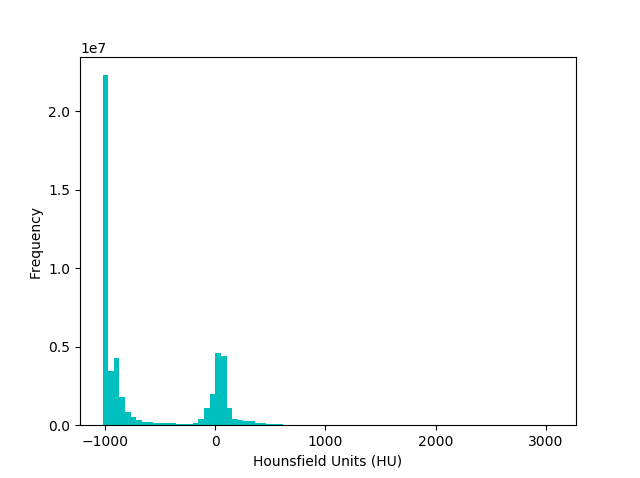
\includegraphics[width=0.4\linewidth]{figures/plot_hist_hu.png}
      }
    	\hspace{0.02\linewidth}
      \subfloat[A screen shot of the game after one swipe right. Note the merge of the two 2-tiles and the random generation of the 2-tile below.]{
          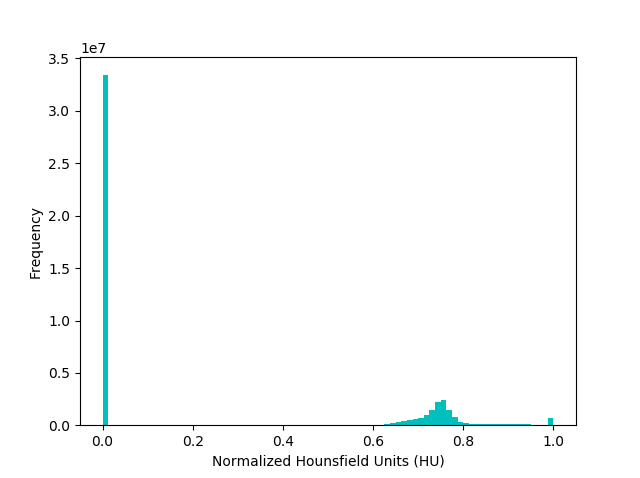
\includegraphics[width=0.4\linewidth]{figures/plot_hist_norm_hu.png}
      }
      \label{fig:hist}
\end{figure}

\begin{figure}
    \centering
         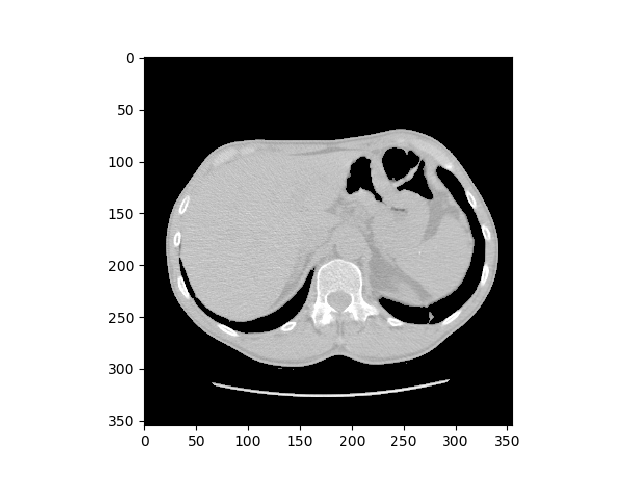
\includegraphics[width=0.8\linewidth]{figures/plot_slice.png}
      \label{fig:slice}
\end{figure}

\begin{figure}
    \centering
      \subfloat[A screen shot of an initial game state.] {
         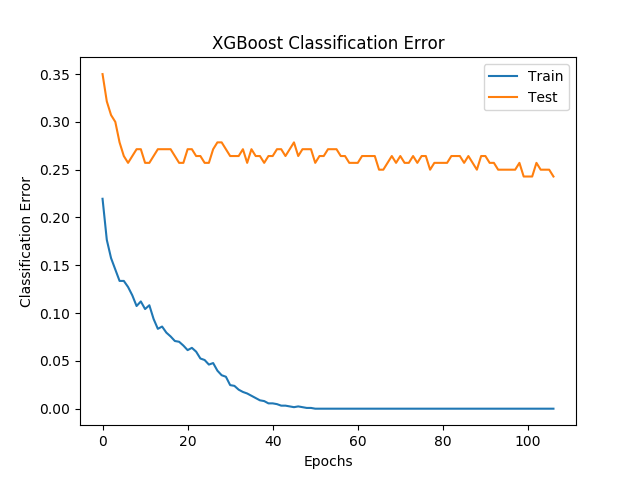
\includegraphics[width=0.4\linewidth]{figures/plot_training_error.png}
      }
    	\hspace{0.02\linewidth}
      \subfloat[A screen shot of the game after one swipe right. Note the merge of the two 2-tiles and the random generation of the 2-tile below.]{
          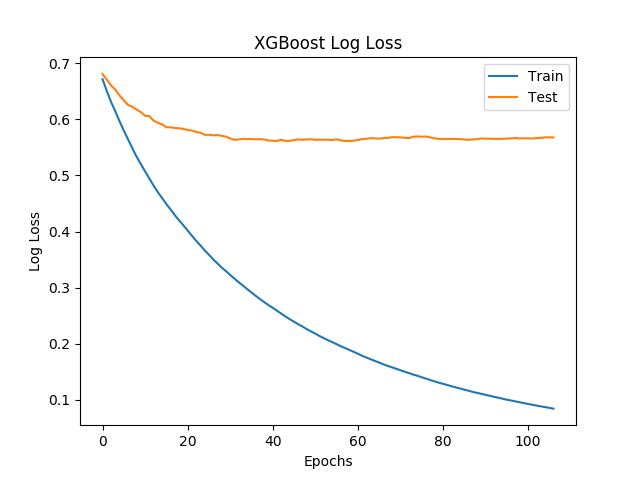
\includegraphics[width=0.4\linewidth]{figures/plot_training_logloss.png}
      }
      \label{fig:training}
\end{figure}

\begin{figure}
    \centering
      \subfloat[A screen shot of an initial game state.] {
         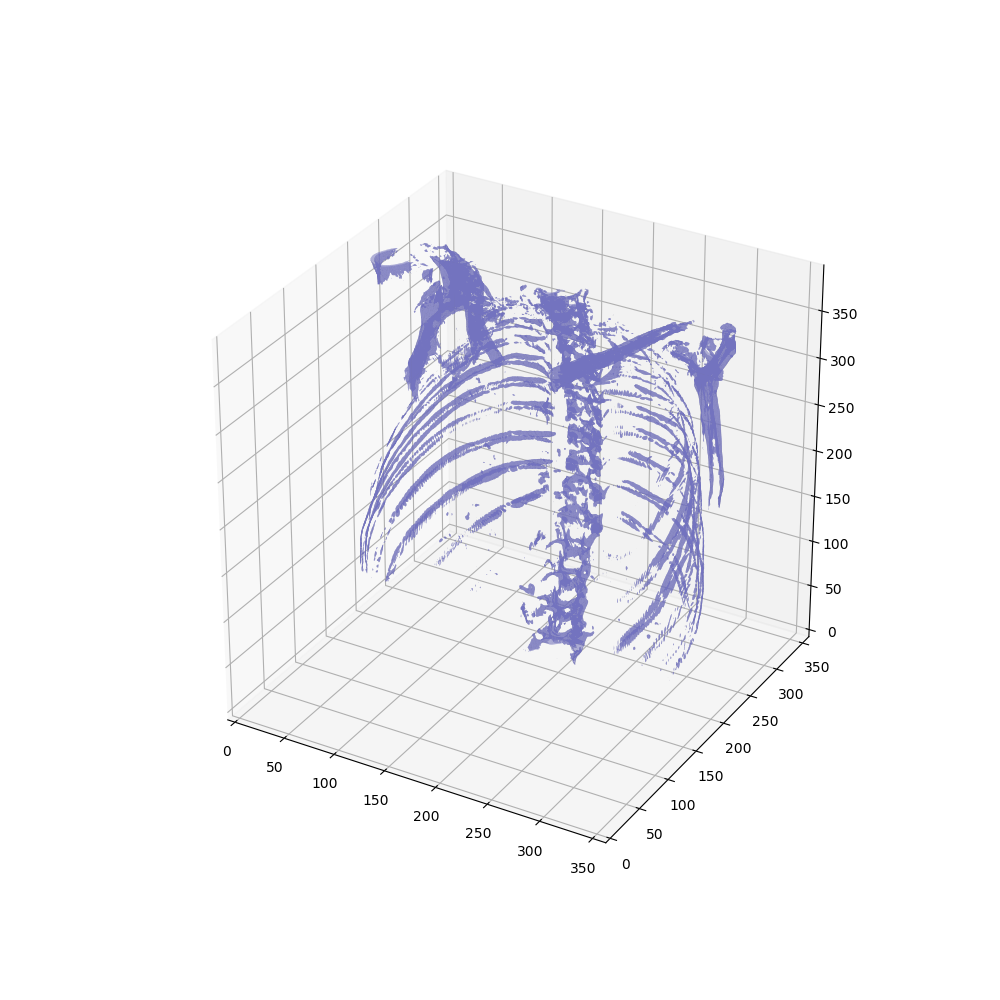
\includegraphics[width=0.4\linewidth]{figures/plot_bones.png}
      }
    	\hspace{0.02\linewidth}
      \subfloat[A screen shot of the game after one swipe right. Note the merge of the two 2-tiles and the random generation of the 2-tile below.]{
          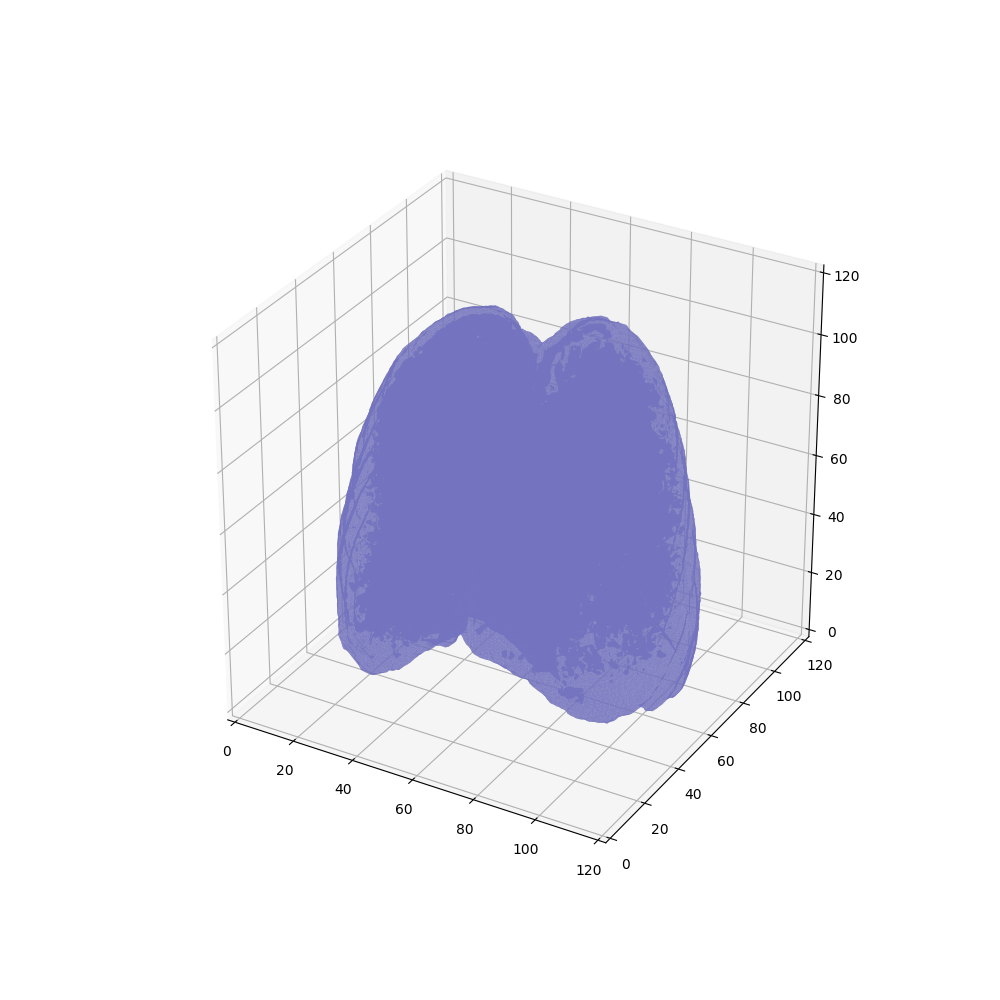
\includegraphics[width=0.4\linewidth]{figures/plot_lungs.png}
      }
      \label{fig:hist}
\end{figure}

\begin{figure}
    \centering
         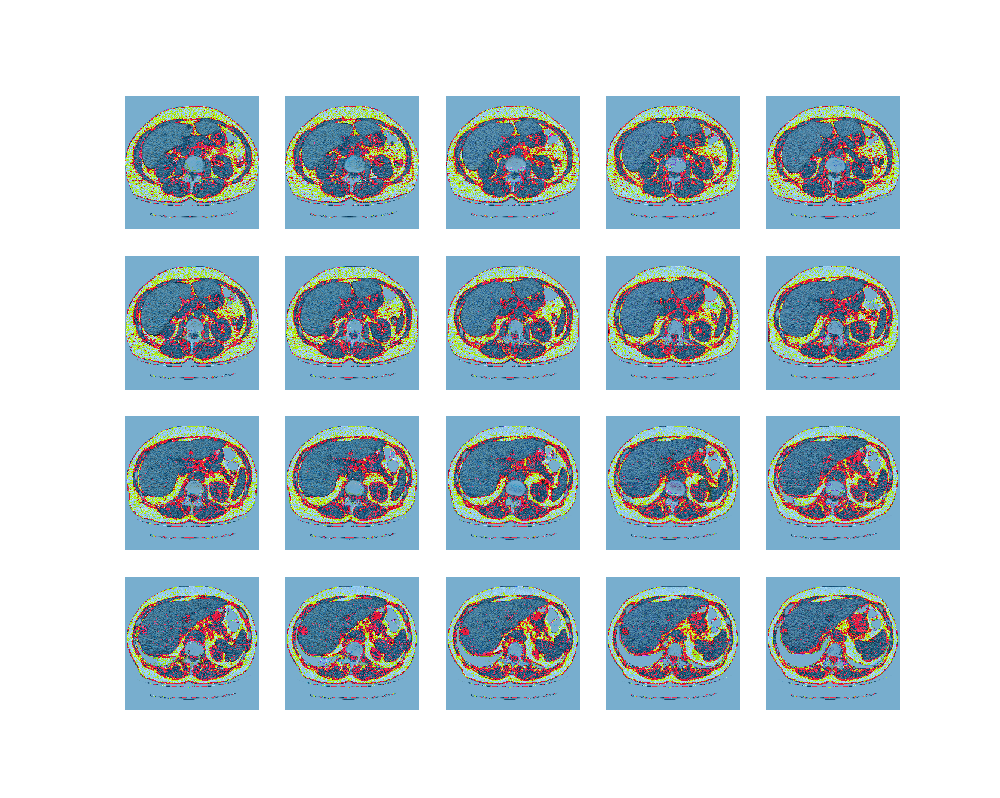
\includegraphics[width=0.8\linewidth]{figures/plot_slices.png}
      \label{fig:slices}
\end{figure}

%\onecolumn
%\section{Appendix A}

\bibliography{myrefs}
\bibliographystyle{IEEEtran}

\end{document}

